\documentclass[a4paper]{beamer}
\usepackage[utf8]{inputenc}
\usepackage{listings}
\usepackage{ textcomp }
\usepackage[absolute,overlay]{textpos}
\graphicspath{{img/}}
\usetheme{Madrid}
\usecolortheme{crane}
\useoutertheme{shadow}
\usefonttheme{structurebold}
\setbeamertemplate{navigation symbols}{}%remove navigation symbols

\definecolor{applegreen}{rgb}{0.55, 0.71, 0.0}
\definecolor{applegreenpale}{rgb}{0.75, 0.91, 0.2}

\title[Migrating to a NFV-based Home Gateway : the SvNF approach] % (optional, only for long titles)
{Migrating to a NFV-based Home Gateway}
\subtitle{Introducing a Surrogate vNF approach}
\author[\underline{Herbaut}, Negru, Xilouris, Chen] % (optional, for multiple authors)
{\underline{N.~Herbaut\inst{1}} \and D.~Négru\inst{1} \and G.~Xilouris\inst{2} \and Y.Chen\inst{3} }
\institute[Universities Here and There] % (optional)
{
  \inst{1}%
  CNRS, LaBRI Lab.\\
  Université de Bordeaux, France
  \and
  \inst{2}%
  NCSR Demokritos\\
  Athens, Greece
  \and
  \inst{3}%
  Orange Labs\\
  Issy-les-moulineaux, France 
}
\date[KPT 2004] % (optional)
{The 6th International Conference On Network of the Future}
\subject{Computer Science.}

\begin{document}
\frame{\titlepage}


\begin{frame}{Objectives of the paper}
									
	\begin{itemize}
																	
		\item Proposing a technical solution to ease the migration to future Home Gateway technologies.
		      \pause
		\item Study the feasibility through a concrete usecase.
	\end{itemize}
									
									
\end{frame}

%%%%%%%%%%%%%%%%%%%%%%%%%%%%%%%%%%%%%%%%%%%%%%%%%%%%%%%%%%%%%%%%%%
%%%%%%%%%%%%%%%%%%%%%%%%%%%%%%%%%%%%%%%%%%%%%%%%%%%%%%%%%%%%%%%%%%
%%%%%%%%%%%%%%%%%%%%%%%%%%%%%%%%%%%%%%%%%%%%%%%%%%%%%%%%%%%%%%%%%%
%%%%%%%%%%%%%%%%%%%%%%%%%%%%%%%%%%%%%%%%%%%%%%%%%%%%%%%%%%%%%%%%%%

\begin{frame}{Presentation plan}
															
															
														
	\begin{columns}[c] % the "c" option specifies center vertical alignment
		\column{.03\textwidth} % column designated by a command
		\begin{block}{}
			\rotatebox{90}{~~~~~Context~~~~~~}
		\end{block}
		\column{.25\textwidth} % column designated by a command
		\begin{block}{1. Home Boxes Today}
			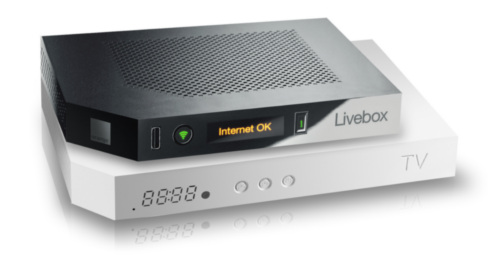
\includegraphics[width= \textwidth]{homebox.jpg}
		\end{block}
		\column{.25\textwidth}
		\begin{block}{2. Virtual Home Gateway }
			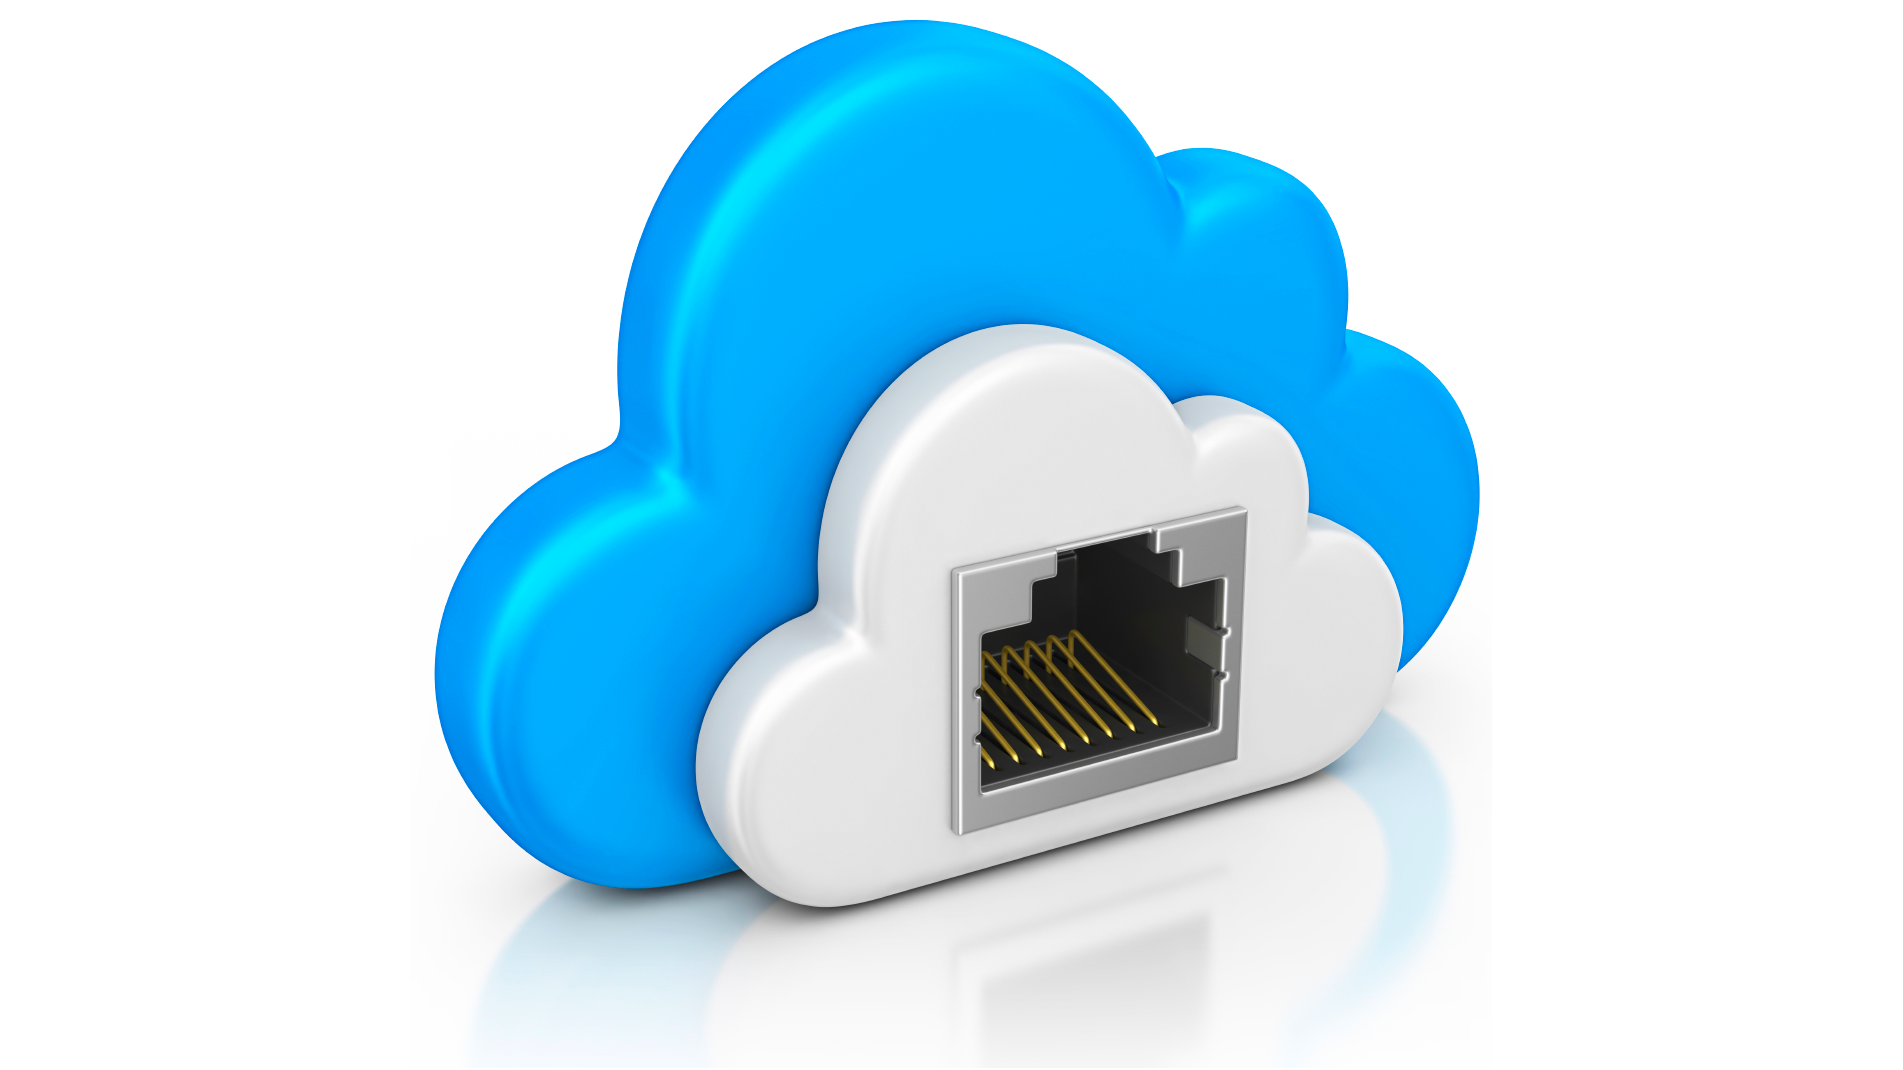
\includegraphics[width= \textwidth]{vhg.png}
		\end{block}
																												          
		\column{.25\textwidth}
		\begin{block}{3. NFV for Future Networks}
			
\includegraphics[width= \textwidth]{etsinfv.png}
		\end{block}
																												          
																												      
	\end{columns}
													
	\setbeamercolor{block title}{bg=applegreen}
													
														    
	\begin{columns}[c] % the "c" option specifies center vertical alignment
		\column{.03\textwidth} % column designated by a command
		\begin{block}{}
			\rotatebox{90}{~~~~Proposal~~~~~}
		\end{block}
																										
		\column{.25\textwidth} % column designated by a command
		\begin{block}{4. Easing the Migration}
			
\includegraphics[width= \textwidth]{loco.png}
		\end{block}
																												 
		\column{.25\textwidth} % column designated by a command
		\begin{block}{5. Experiments, Results}
			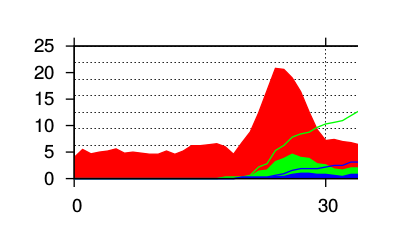
\includegraphics[width= \textwidth]{results.png}
		\end{block}
																												          
		\column{.25\textwidth} % column designated by a command
		\begin{block}{6. Discussion \& Conclusion}
			
\includegraphics[width= \textwidth]{etsinfv.png}
		\end{block}
																												 
	\end{columns}
														    
												
														    
														    
\end{frame}


%%%%%%%%%%%%%%%%%%%%%%%%%%%%%%%%%%%%%%%%%%%%%%%%%%%%%%%%%%%%%%%%%%
%%%%%%%%%%%%%%%%%%%%%%%%%%%%%%%%%%%%%%%%%%%%%%%%%%%%%%%%%%%%%%%%%%
%%%%%%%%%%%%%%%%%%%%%%%%%%%%%%%%%%%%%%%%%%%%%%%%%%%%%%%%%%%%%%%%%%
%%%%%%%%%%%%%%%%%%%%%%%%%%%%%%%%%%%%%%%%%%%%%%%%%%%%%%%%%%%%%%%%%%

\begin{frame}{With Customer Permise Equipment (CPE), Service Providers bring a lot of features to Users}
										
									
	\begin{columns}[T] 
		\begin{column}[T]{0.25 \textwidth} 
			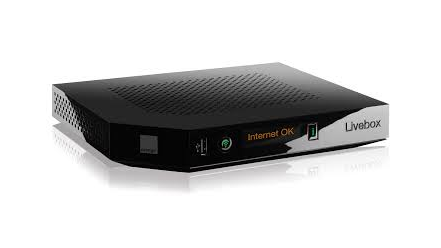
\includegraphics[width=\linewidth]{livebox.png}
		\end{column}
																						
		\begin{column}[T]{0.75 \textwidth} % each column can also be its own environment
																																	
			\textbf{Home Gateway  (HG)}
			\begin{itemize}
				\item Connects the Service Provider Network 
				\item Network services: NAT, DHCP, Wifi...
				\item Users-facing services: Printing Service, VoIP, Parental Control...
				\item New Services: Internet of Things, Home Automation...
			\end{itemize}
			\vspace{1em}
																																	
		\end{column}
																						
	\end{columns}
										
										
											
										
	\begin{columns}[T] 
		\begin{column}[T]{0.25 \textwidth} 
			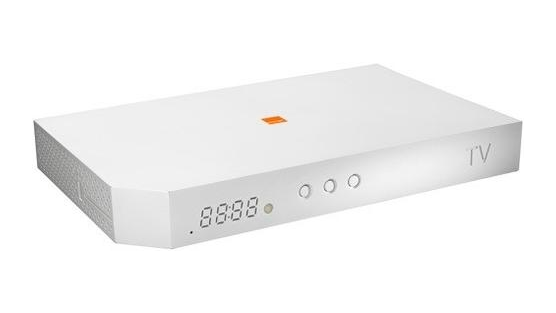
\includegraphics[width=\linewidth]{liveboxdec.png}
		\end{column}
																						
		\begin{column}[T]{0.75 \textwidth} % each column can also be its own environment
																																	
																																		   
			\textbf{ Set-Top-Box (STB)}
			\begin{itemize}
				\item Decode media IP flows to a display device (through HDMI)
				\item Live TV, Video On Demand ...
				\item Catch-up TV, Recording ...
				\item Legacy Digital terrestrial television ...
			\end{itemize}
																																		     
																																	
		\end{column}
																						
	\end{columns}
											
											
											
\end{frame}

%%%%%%%%%%%%%%%%%%%%%%%%%%%%%%%%%%%%%%%%%%%%%%%%%%%%%%%%%%%%%%%%%%
%%%%%%%%%%%%%%%%%%%%%%%%%%%%%%%%%%%%%%%%%%%%%%%%%%%%%%%%%%%%%%%%%%
%%%%%%%%%%%%%%%%%%%%%%%%%%%%%%%%%%%%%%%%%%%%%%%%%%%%%%%%%%%%%%%%%%
%%%%%%%%%%%%%%%%%%%%%%%%%%%%%%%%%%%%%%%%%%%%%%%%%%%%%%%%%%%%%%%%%%

\begin{frame}{CPEs cost a lot to produce and to support}
									
	\begin{columns}[T] 
		\begin{column}[T]{0.15 \textwidth} 
			
\includegraphics[width=3em]{bagofmoney.jpg}
		\end{column}
																						
		\begin{column}[T]{0.75 \textwidth} % each column can also be its own environment
																																	
																																		   
			\textbf{ High Capital Expenditure (CAPEX)}
			\begin{itemize}
				\item High design \& Engineering costs
				\item Supply Chain costs, need for spare devices
				\item Hardware upgrades can be necessary to rollout new services
			\end{itemize}
			\vspace{3em}				     
																																	
		\end{column}
																						
	\end{columns}
									
									
	\begin{columns}[T] 
		\begin{column}[T]{0.15 \textwidth} 
			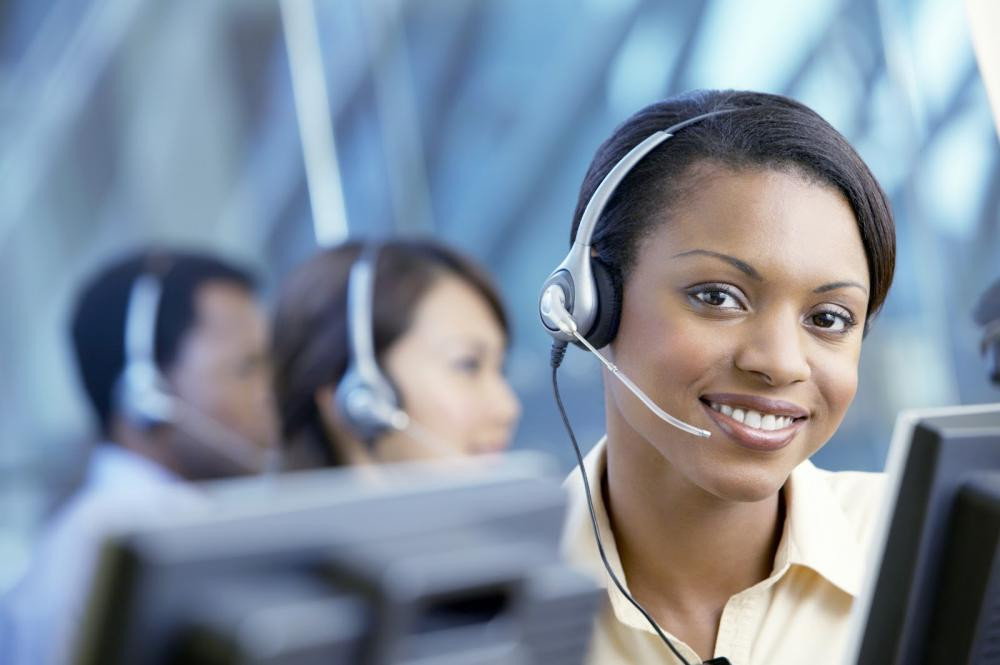
\includegraphics[width=6em]{customer-care.jpg}
		\end{column}
																		
																						
		\begin{column}[T]{0.75 \textwidth} % each column can also be its own environment
																																	
																																		   
			\textbf{ High Operational Expenditure (OPEX)}
			\begin{itemize}
				\item Need to maintain legacy models
				\item Difficult to update software of a very fragmented installed base
				\item Costly customer service 
			\end{itemize}
																																		     
																																	
		\end{column}
																						
	\end{columns}
									
									
\end{frame}


%%%%%%%%%%%%%%%%%%%%%%%%%%%%%%%%%%%%%%%%%%%%%%%%%%%%%%%%%%%%%%%%%%
%%%%%%%%%%%%%%%%%%%%%%%%%%%%%%%%%%%%%%%%%%%%%%%%%%%%%%%%%%%%%%%%%%
%%%%%%%%%%%%%%%%%%%%%%%%%%%%%%%%%%%%%%%%%%%%%%%%%%%%%%%%%%%%%%%%%%
%%%%%%%%%%%%%%%%%%%%%%%%%%%%%%%%%%%%%%%%%%%%%%%%%%%%%%%%%%%%%%%%%%

\begin{frame}{CPEs cost a lot to produce and to support}
									
	\begin{columns}[T] 
		\begin{column}[T]{0.15 \textwidth} 
			
\includegraphics[width=3em]{bagofmoney.jpg}
		\end{column}
																						
		\begin{column}[T]{0.75 \textwidth} % each column can also be its own environment
																																	
																																		   
			\textbf{ High Capital Expenditure (CAPEX)}
			\begin{itemize}
				\item High design \& Engineering costs
				\item Supply Chain costs, need for spare devices
				\item Hardware upgrades can be necessary to rollout new services
			\end{itemize}
			\vspace{3em}				     
																																	
		\end{column}
																						
	\end{columns}
									
									
	\begin{columns}[T] 
		\begin{column}[T]{0.15 \textwidth} 
			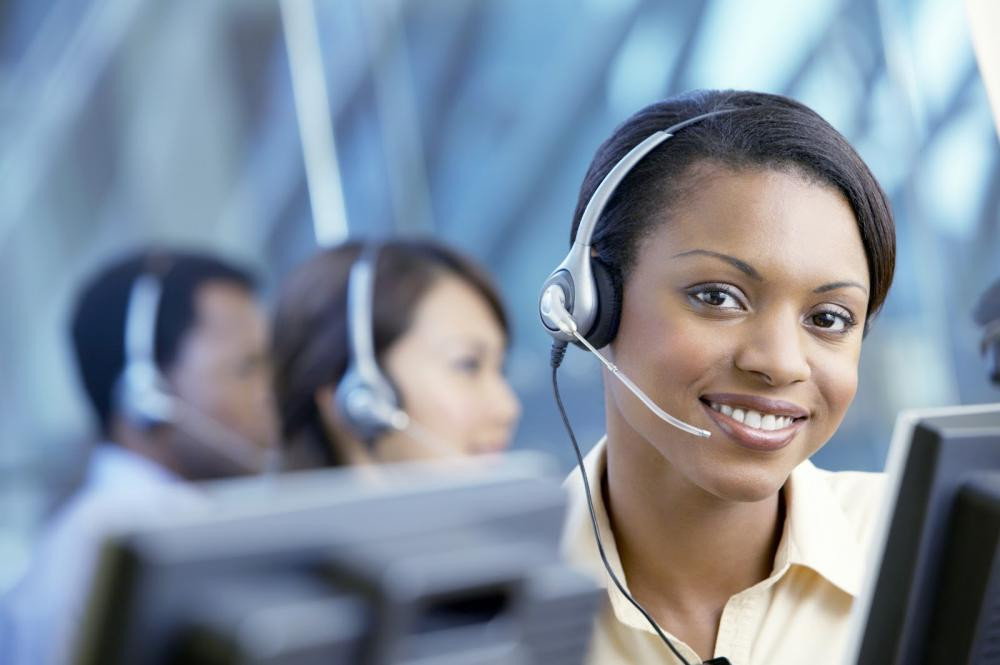
\includegraphics[width=6em]{customer-care.jpg}
		\end{column}
																		
																						
		\begin{column}[T]{0.75 \textwidth} % each column can also be its own environment
																																	
																																		   
			\textbf{ High Operational Expenditure (OPEX)}
			\begin{itemize}
				\item Need to maintain legacy models
				\item Difficult to update software of a very fragmented installed base
				\item Costly customer service 
			\end{itemize}
																																		     
																																	
		\end{column}
																						
	\end{columns}
									
								
	\begin{textblock*}{10cm}(1cm,0.5\textheight)
		\begin{alertblock}{}
			\textbf{  How do we fix it? }
			\begin{itemize}
				\item Can we design better CPE architecure?
				\item Can we simplyfy the deployment of new services?
				\item Can we leverage existing industry proposals?
			\end{itemize}
		\end{alertblock}
	\end{textblock*}
									
\end{frame}

\begin{frame}{Current CPE architectures are not modular: maintenance and new service deployement are hard.}
								
	\begin{columns}[T]
		\begin{column}{.01\textwidth} % column designated by a command
			\rotatebox{90}{~~~~Monolithic~~~~}
		\end{column}
		\begin{column}[T]{0.15 \textwidth} 
			\vspace{1em}
			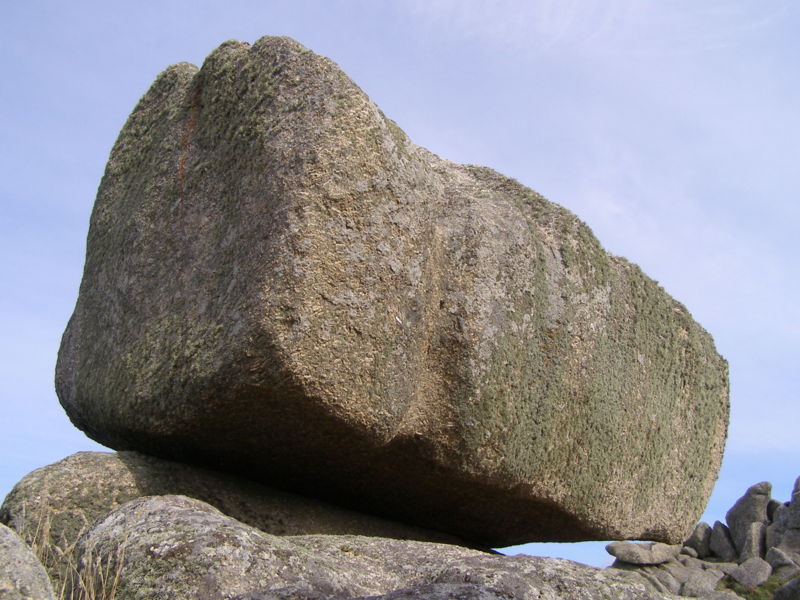
\includegraphics[width=6em]{monolith.jpg}
		\end{column}
																		
																						
		\begin{column}[T]{0.70 \textwidth} 
																																	
																																		   
			\textbf{Today: Firmware-based Home Gateways}
			\begin{itemize}
				\item Embded system software
				\item Complete system update to deploy new feature
				\item Still widely used by vendors
			\end{itemize}
			\vspace{5mm}
																																		     
																																	
		\end{column}
																						
	\end{columns}
								
							
									
\end{frame}


\begin{frame}{Alternative Modular CPE architectures exist, new service can be pushed easily}
					
					
	\begin{columns}[T]
		\begin{column}{.01\textwidth} % column designated by a command
			\rotatebox{90}{~~~~Modular~~~~}
		\end{column}
		\begin{column}[T]{0.15 \textwidth} 
			\vspace{1em}
			
\includegraphics[width=4em]{tux.png}
		\end{column}
																		
																						
		\begin{column}[T]{0.70 \textwidth} 
																																	
																																		   
			\textbf{ GNU/Linux Home Gateways}
			\begin{itemize}
				\item Stable, tested, reusable codebase
				\item Modularity through package management
				\item Limited support for Service Oriented Architecture
			\end{itemize}
			\vspace{3mm}
																																		     
																																	
		\end{column}
																						
	\end{columns}
						
						
	\begin{columns}[T]
		\begin{column}{.01\textwidth} % column designated by a command
			\rotatebox{90}{~~~~Modular~~~~}
		\end{column}
		\begin{column}[T]{0.15 \textwidth} 
			\vspace{2em}
			
\includegraphics[width=6em]{hgi.png}
		\end{column}
																		
																						
		\begin{column}[T]{0.70 \textwidth} 
																																	
																																		   
			\textbf{ HGI Open Platform 2.0}
			\begin{itemize}
				\item Support OSGI Standard for modularity
				\item Support mainly JVM dialects
				\item Service Oriented Architecture
			\end{itemize}
			\vspace{3mm}
																																		     
																																	
		\end{column}
																						
	\end{columns}
				
				
	\begin{columns}[T]
		\begin{column}{.01\textwidth} % column designated by a command
											
			\rotatebox{90}{~~~~Modular~~~~}
		\end{column}
		\begin{column}[T]{0.15 \textwidth} 
			\vspace{1em}
			
\includegraphics[width=4em]{droid.png}
		\end{column}
																		
																						
		\begin{column}[T]{0.70 \textwidth} 
																																	
																																		   
			\textbf{ Android}
			\begin{itemize}
				\item Thousands of applications
				\item Designed for multi-vendor
				\item Service Oriented Architecture
			\end{itemize}
			\vspace{5mm}
																																		     
																																	
		\end{column}
																						
	\end{columns}
					
						
						
						
								
						
							
\end{frame}



\begin{frame}{Alternative Modular CPE architectures exist, new service can be pushed easily}
					
					
	\begin{columns}[T]
		\begin{column}{.01\textwidth} % column designated by a command
			\rotatebox{90}{~~~~Modular~~~~}
		\end{column}
		\begin{column}[T]{0.15 \textwidth} 
			\vspace{1em}
			
\includegraphics[width=4em]{tux.png}
		\end{column}
																		
																						
		\begin{column}[T]{0.70 \textwidth} 
																																	
																																		   
			\textbf{ GNU/Linux Home Gateways}
			\begin{itemize}
				\item Stable, tested, reusable codebase
				\item Modularity through package management
				\item Limited support for Service Oriented Architecture
			\end{itemize}
			\vspace{3mm}
																																		     
																																	
		\end{column}
																						
	\end{columns}
						
						
	\begin{columns}[T]
		\begin{column}{.01\textwidth} % column designated by a command
			\rotatebox{90}{~~~~Modular~~~~}
		\end{column}
		\begin{column}[T]{0.15 \textwidth} 
			\vspace{2em}
			
\includegraphics[width=6em]{hgi.png}
		\end{column}
																		
																						
		\begin{column}[T]{0.70 \textwidth} 
																																	
																																		   
			\textbf{ HGI Open Platform 2.0}
			\begin{itemize}
				\item Support OSGI Standard for modularity
				\item Support mainly JVM dialects
				\item Service Oriented Architecture
			\end{itemize}
			\vspace{3mm}
																																		     
																																	
		\end{column}
																						
	\end{columns}
				
				
	\begin{columns}[T]
		\begin{column}{.01\textwidth} % column designated by a command
											
			\rotatebox{90}{~~~~Modular~~~~}
		\end{column}
		\begin{column}[T]{0.15 \textwidth} 
			\vspace{1em}
			
\includegraphics[width=4em]{droid.png}
		\end{column}
																		
																						
		\begin{column}[T]{0.70 \textwidth} 
																																	
																																		   
			\textbf{ Android}
			\begin{itemize}
				\item Thousands of applications
				\item Designed for multi-vendor
				\item Service Oriented Architecture
			\end{itemize}
			\vspace{5mm}
																																		     
																																	
		\end{column}
																						
	\end{columns}
					
						
						
					
	\begin{textblock*}{7cm}(3cm,0.5\textheight)
		\begin{alertblock}{}
			\textbf{  We didn't fix the major issues. }
			\begin{itemize}
				\item Deploying new software is easier, but still difficult due to the scale.
				\item CAPEX and OPEX are still high.
				\item We may need to replace the whole CPE due to hardware limitations.
			\end{itemize}
		\end{alertblock}
	\end{textblock*}			
									
							
								
\end{frame}

\begin{frame}{Virtual CPE is an alternative and disruptive scenario}
				
	\begin{columns}[T]
		\begin{column}[T]{0.33 \textwidth} 
			\vspace{2.2cm}
			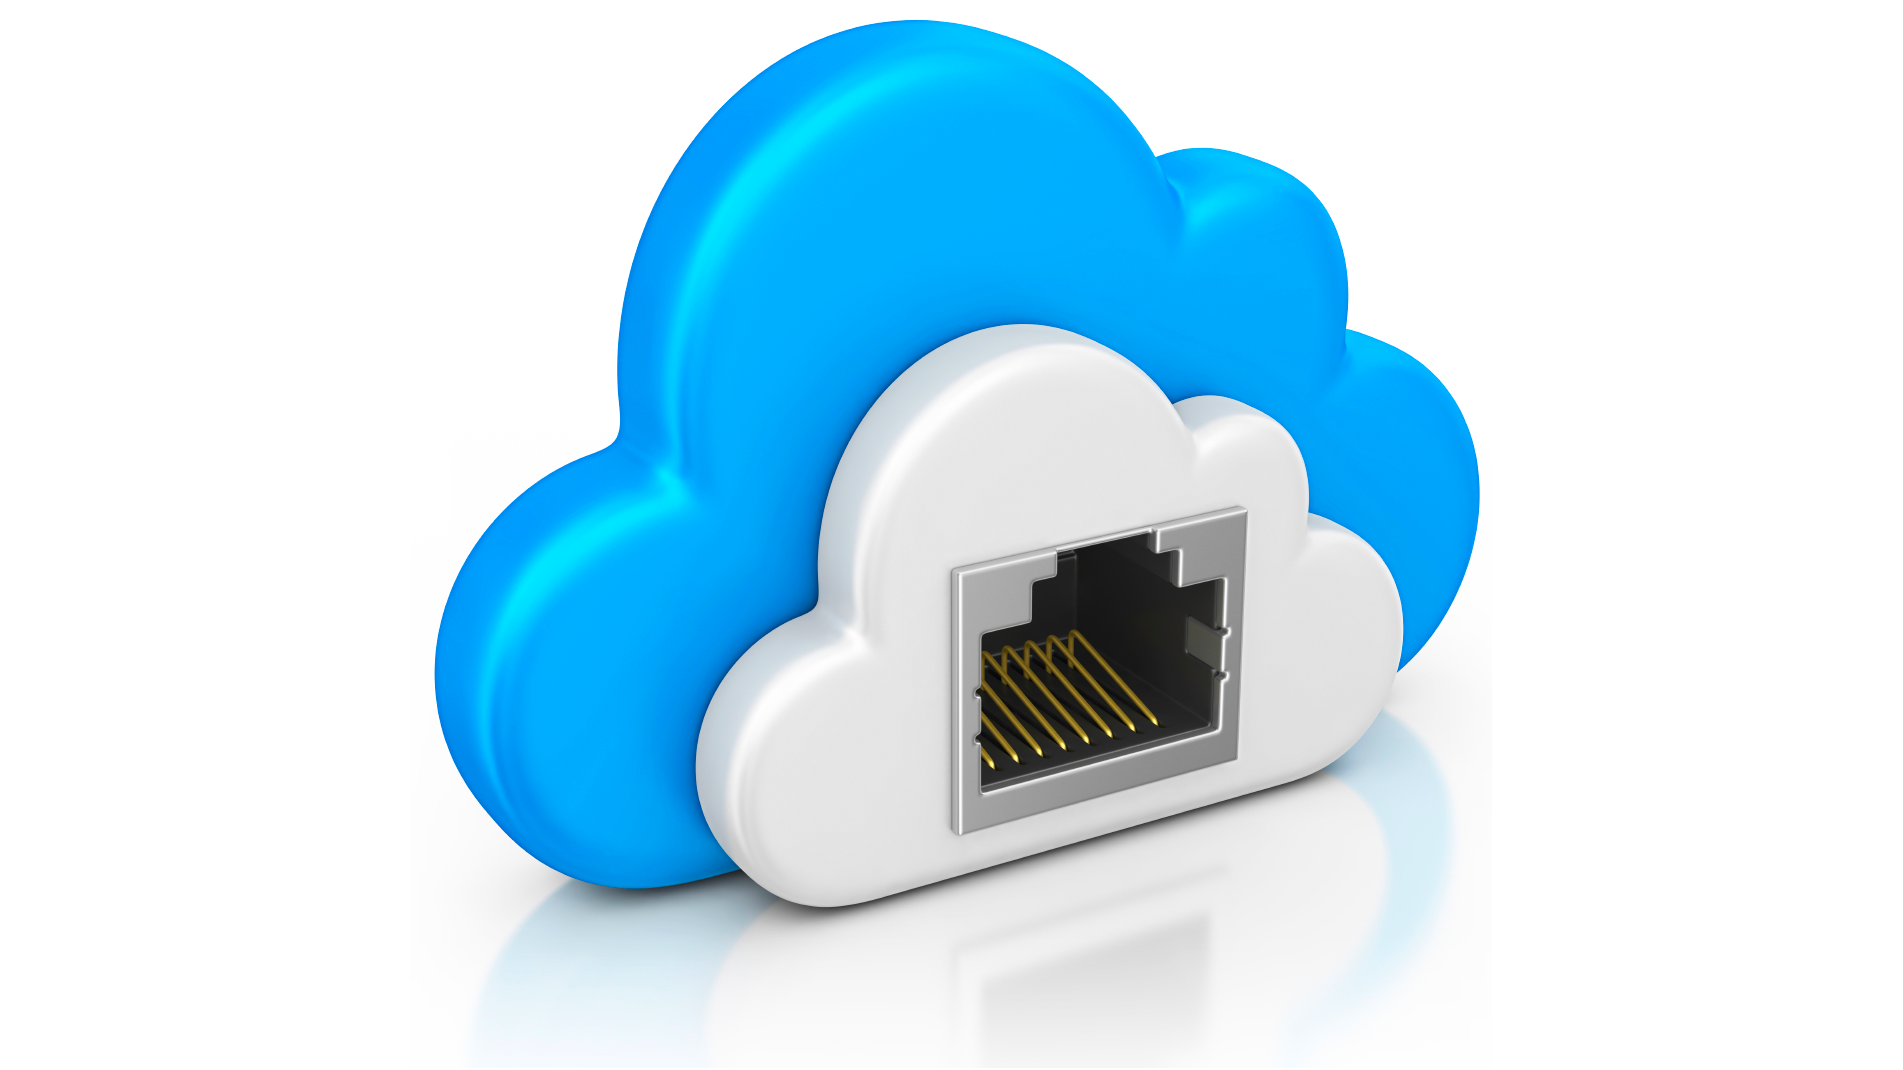
\includegraphics[width=12em]{vhg.png}
		\end{column}
						
		\begin{column}[T]{0.66\textwidth} 
				   
			\textbf{ Virtual CPE}
			\begin{itemize}
				\item Pulling network functions into the operator network
				\item Shared Resources, optimized dimentionning
				\item Managing $O(10^{3})$ Network Nodes is easier than $O(10^{6})$ of CPE.
			\end{itemize}
			\vspace{3mm}
			\textbf{General Approach}
			\begin{itemize}
				\item Replacing existing HG by a Layer-2 device, handling VoIP and Wifi.
				\item Current functions (NAT and DHCP) are realized in the operator network
				\item The Virtual Home Gateway can be used in mobility 
			\end{itemize}
				
																																
		\end{column}
																						
	\end{columns}
								
\end{frame}

\begin{frame}{Several Architecture are proposed by Research.}
		
	\begin{columns}[T]
		\begin{column}[T]{0.33 \textwidth} 
									
			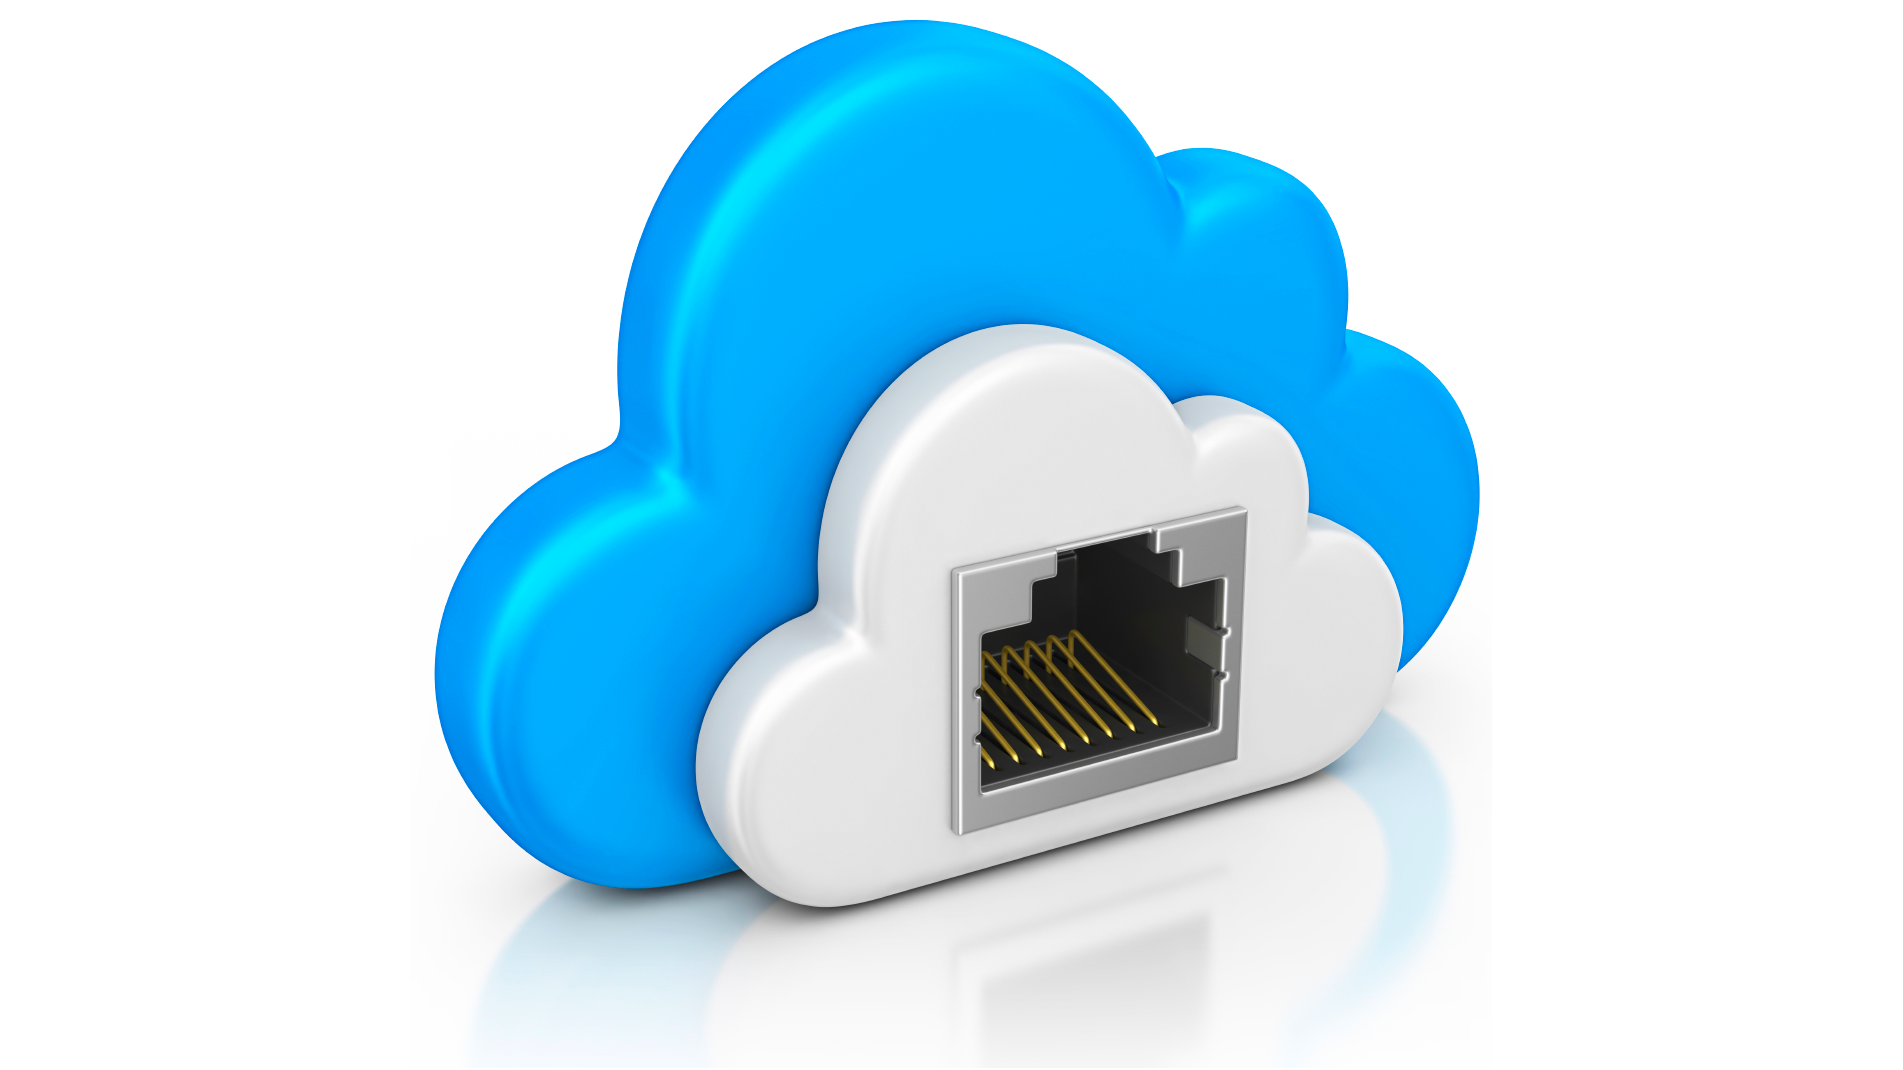
\includegraphics[width=12em]{vhg.png}
		\end{column}
						
		\begin{column}[T]{0.66\textwidth} 
				   
					\textbf{Characteristics of the different approaches}
					\begin{itemize}
						\item What do we remove from HG?
						\item Where do we operate virtualized services?
						\item How do we virtualized services?
					\end{itemize}
			\vspace{3mm}
																																
		\end{column}
																						
	\end{columns}
		
			
\end{frame}

\begin{frame}[plain,T]{}
	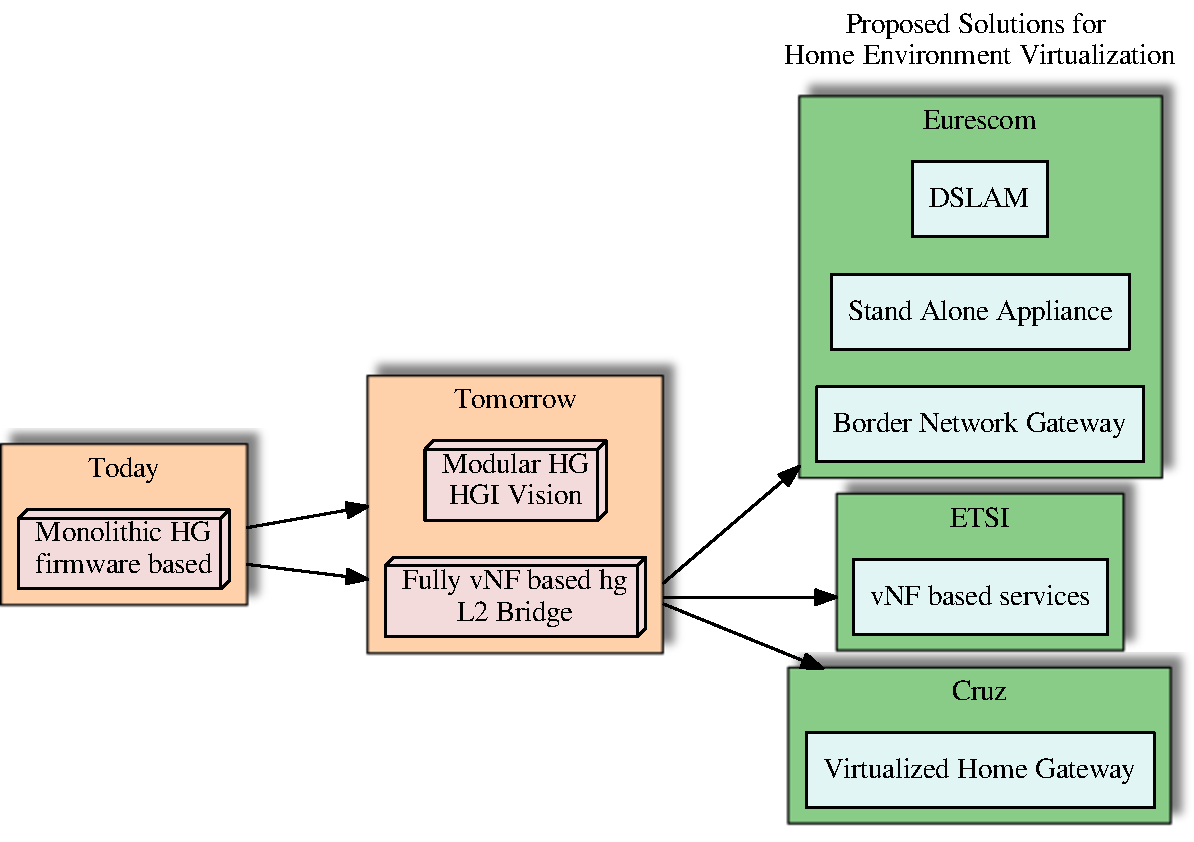
\includegraphics[width=0.9\textwidth]{vhgtrends.pdf}
\end{frame}


\begin{frame}[plain,T]{}
	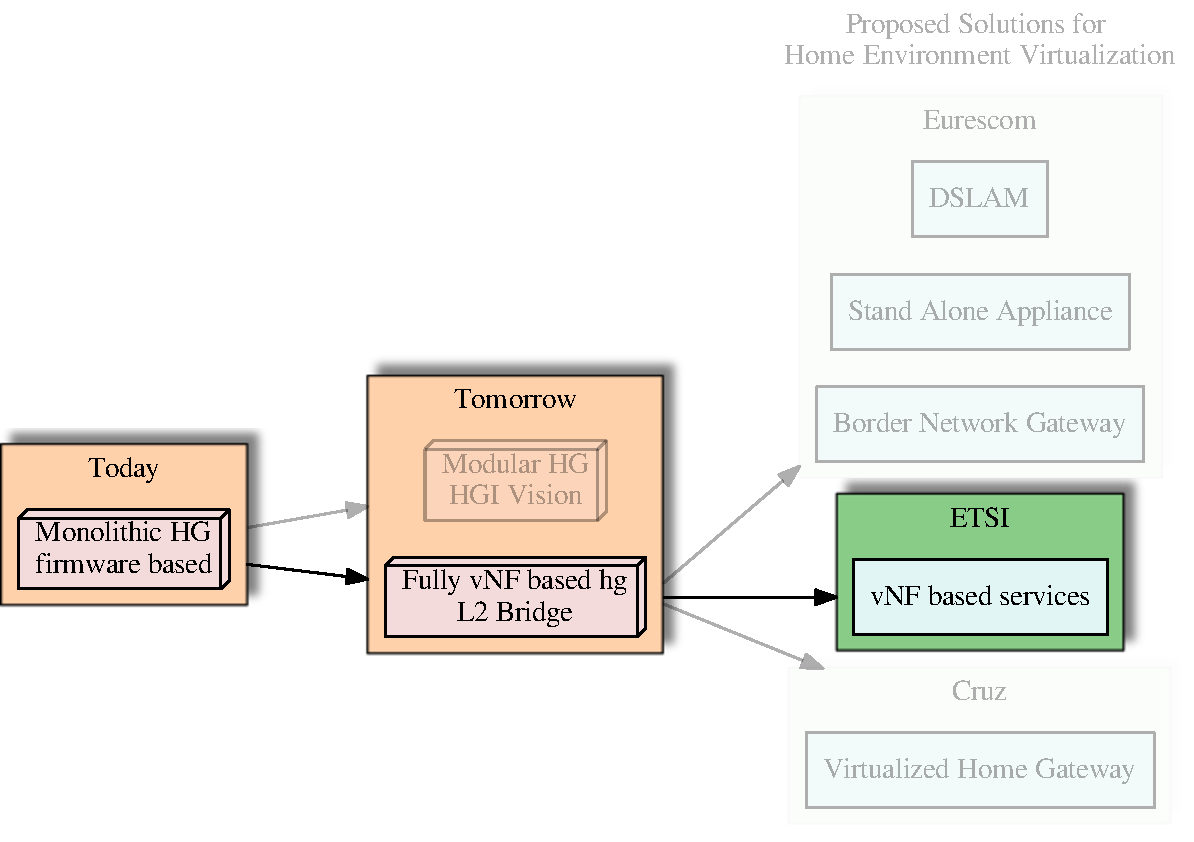
\includegraphics[width=0.9\textwidth]{vhgtrends-etsi-emphasis.pdf}
\end{frame}

\begin{frame}[plain,T]{}
\begin{centering}
	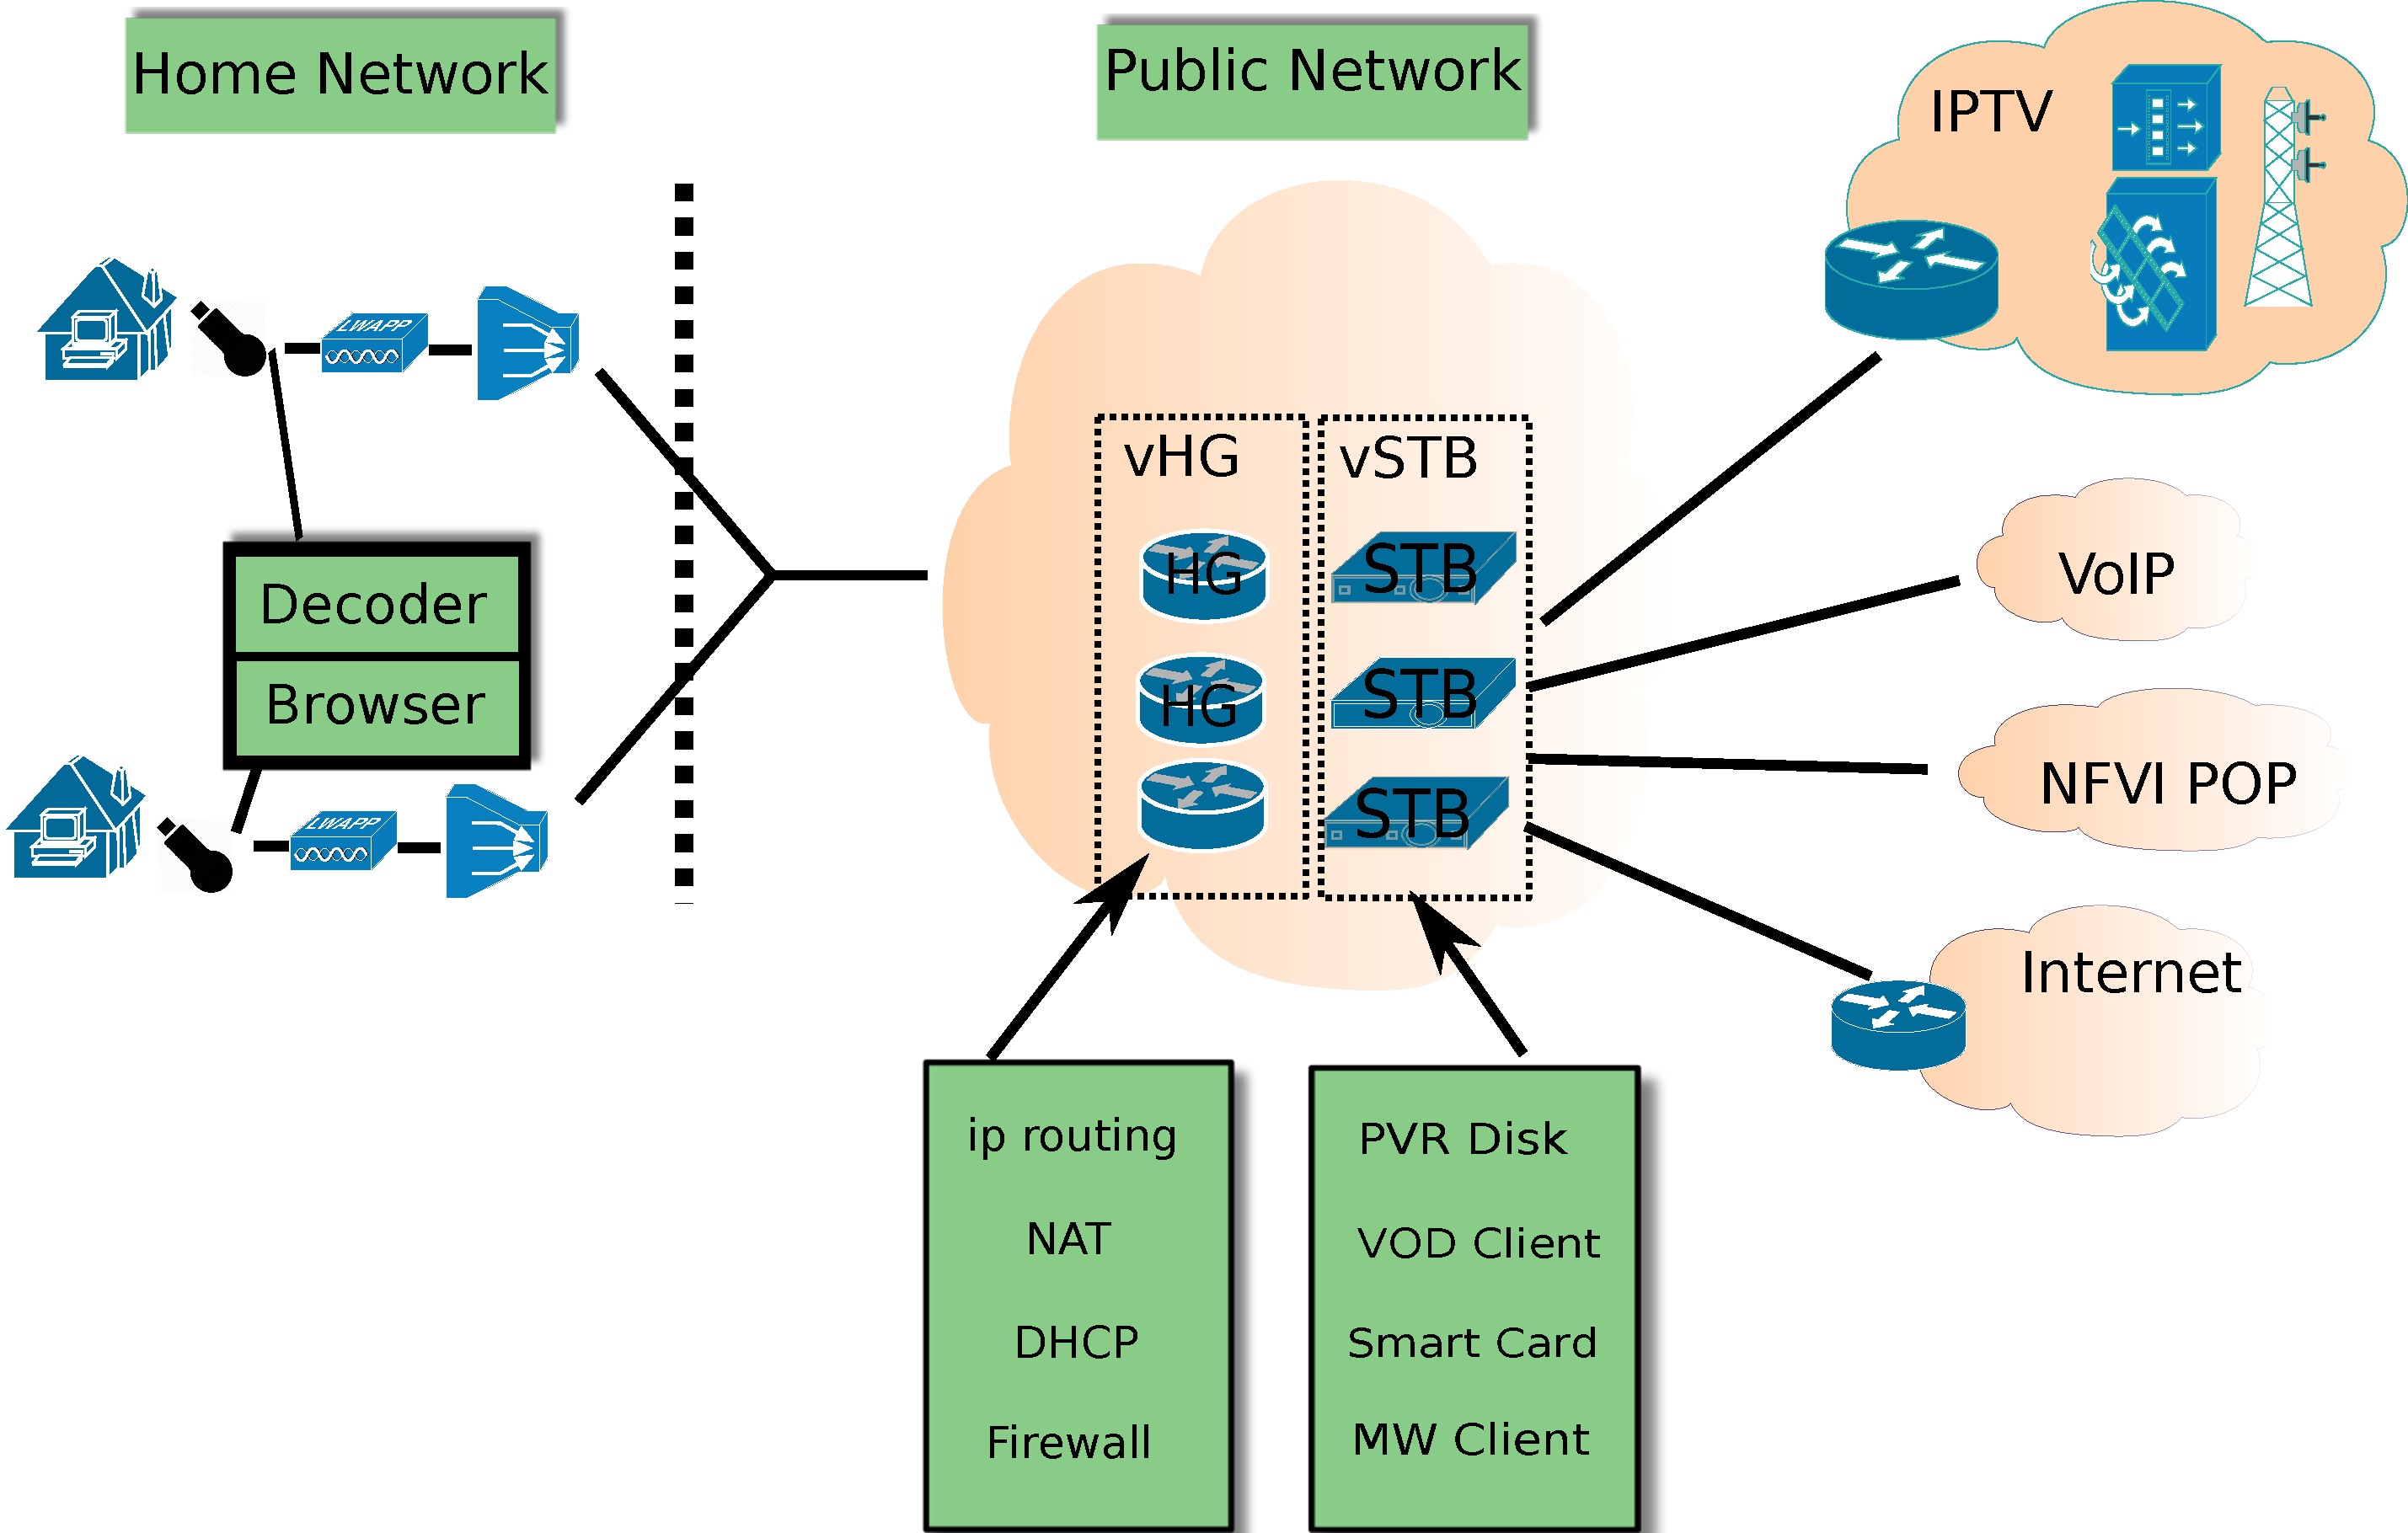
\includegraphics[width=0.9\textwidth]{etsi-virtualisation-home-env.pdf}
\end{centering}
	
\end{frame}




\begin{frame}{Network Function Virtualization (NFV) as a building block for solving vHG issues.}
		\begin{columns}[T]
		\begin{column}[T]{0.33 \textwidth} 
										\vspace{5em}
			
\includegraphics[width=10em]{etsinfv.png}
		\end{column}
						
		\begin{column}[T]{0.66\textwidth} 
				   
					\textbf{ETSI's NFV architecture makes the operator benefits from virtualization}
					\begin{itemize}
						\item Network Functions run on commodity hardware
						\item No more middlebox vendor lock-in
						\item Multivendor nature boost competition and lower prices
						\item Ongoing standardization efforts
					\end{itemize}
			\vspace{3mm}
																																
		\end{column}
																						
	\end{columns}
\end{frame}

\begin{frame}{vHG with vNF is a clean slate approach, which is an issue for migrating to this model}
		\begin{columns}[T]
		\begin{column}[T]{0.33 \textwidth} 
									\vspace{6em}
			
\includegraphics[width=10em]{etsinfv.png}
		\end{column}
						
		\begin{column}[T]{0.66\textwidth} 
				   
				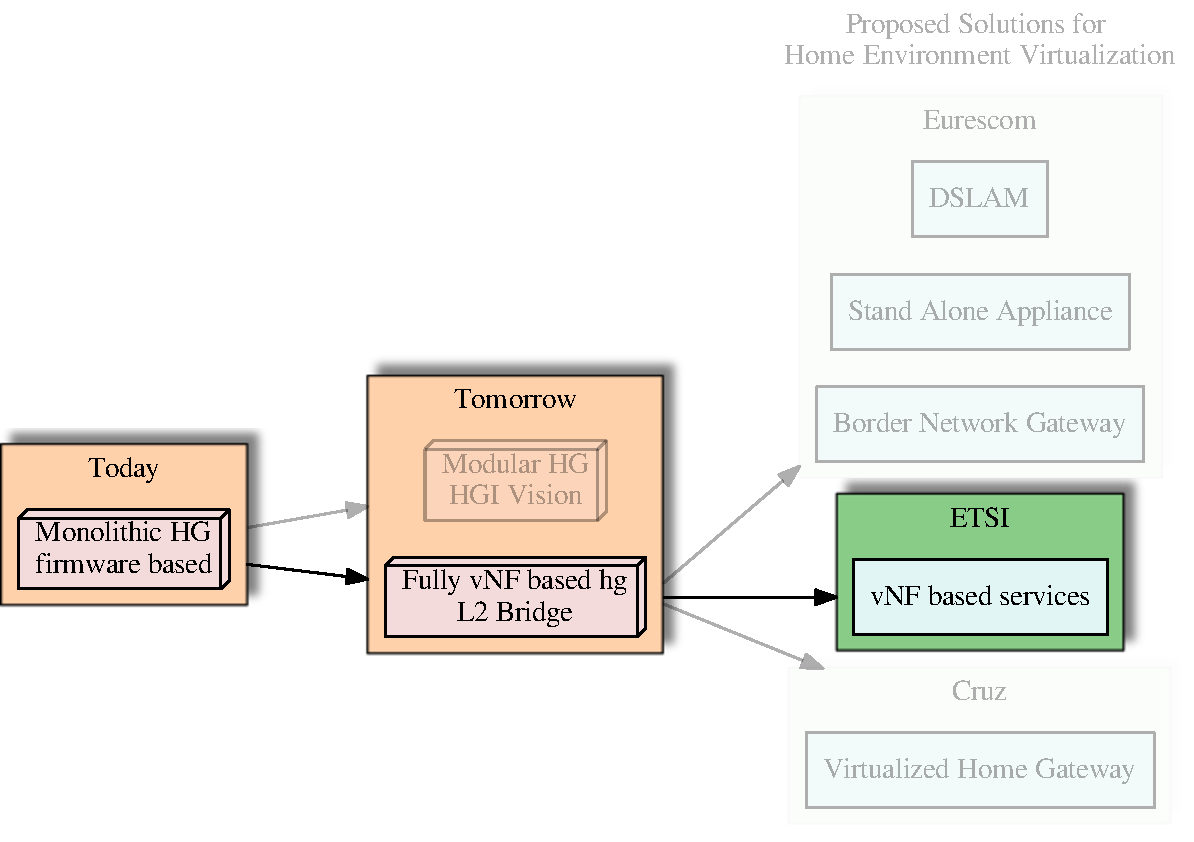
\includegraphics[width=\textwidth]{vhgtrends-etsi-emphasis.pdf}
																																
		\end{column}
																						
	\end{columns}
\end{frame}





\setbeamercolor{frametitle}{bg=applegreen}
\setbeamercolor{frametitle right}{bg=applegreen!90}
\setbeamercolor{footline left}{bg=applegreen}
\setbeamercolor{section in head/foot}{fg=black, bg=applegreen}
\setbeamercolor{title in head/foot}{fg=black, bg=applegreenpale}


\begin{frame}{vHG with vNF is a clean slate approach, which is an issue for migrating to this model}
		\begin{columns}[T]
		\begin{column}[T]{0.33 \textwidth} 
									\vspace{6em}
			
\includegraphics[width=10em]{etsinfv.png}
		\end{column}
						
		\begin{column}[T]{0.66\textwidth} 
				   
				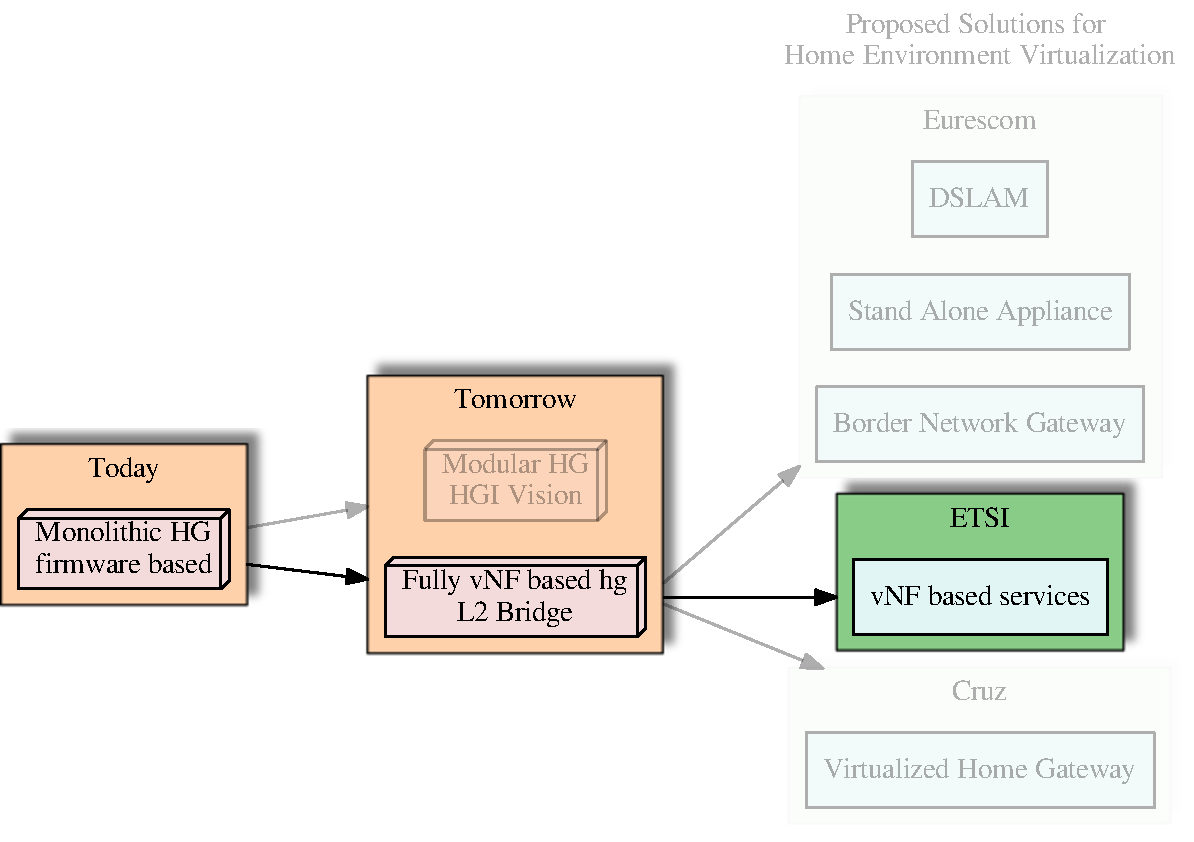
\includegraphics[width=\textwidth]{vhgtrends-etsi-emphasis.pdf}
																																
		\end{column}
																						
	\end{columns}
	\setbeamercolor{block title}{bg=applegreen}
	\begin{textblock*}{8cm}(3cm,0.4\textheight)
		\begin{block}{}
			\textbf{ This is where our contribution help }
			\begin{itemize}
				\item We propose a way to migrate progressively to this final model
				\item We want to start benefitting from NFV as soon as possible
				\item We leverage standards as much as possible
			\end{itemize}
		\end{block}
	\end{textblock*}		
\end{frame}


\begin{frame}{Our contribution eases the migration to vHG}
		\begin{columns}[T]
		\begin{column}[T]{0.33 \textwidth} 
									
			
\includegraphics[width=12em]{loco.png}
		\end{column}
						
		\begin{column}[T]{0.66\textwidth} 
				   
					\textbf{Characteristics of the different approaches}
					\begin{itemize}
						\item What do we remove from HG?
						\item Where do we operate virtualized services?
						\item How do we virtualized services?
					\end{itemize}
			\vspace{3mm}
																																
		\end{column}
																						
	\end{columns}
\end{frame}

\end{document}
